\documentclass[10.5pt,a4paper]{article}
% ---------- layout ----------
\usepackage[a4paper,top=15mm,bottom=16mm,left=17mm,right=17mm]{geometry}
\usepackage[T1]{fontenc}\usepackage[utf8]{inputenc}
\usepackage{charter}\usepackage[scaled=.92]{helvet}
\usepackage{microtype,xcolor,graphicx,tikz,enumitem,titlesec,tabularx,array,fancyhdr,lastpage}
\usepackage{needspace,etoolbox}
\usepackage[hidelinks]{hyperref}
\definecolor{accent}{HTML}{C2401F}\definecolor{ink}{HTML}{1D1B22}\definecolor{mute}{HTML}{6B6672}
\hypersetup{colorlinks=true,urlcolor=accent,linkcolor=accent}
\color{ink}\linespread{1.08}\setlength{\parindent}{0pt}\setlength{\parskip}{0pt}
\pagestyle{fancy}\fancyhf{}\renewcommand{\headrulewidth}{0pt}
\fancyfoot[L]{\footnotesize\color{mute}Satyam Tiwari \textbullet\ Curriculum Vitae}
\fancyfoot[R]{\footnotesize\color{mute}\thepage\,/\,\pageref{LastPage}}
% ---------- sections ----------
\titleformat{\section}{\sffamily\bfseries\large\color{accent}}{}{0pt}{\MakeUppercase}[{\color{accent!35}\titlerule[.6pt]}]
\titlespacing*{\section}{0pt}{11pt}{6pt}
\pretocmd{\section}{\Needspace{7\baselineskip}}{}{}
\setlist[itemize]{leftmargin=1.1em,topsep=2pt,itemsep=1.5pt,parsep=0pt,label={\color{accent}\small\textbullet}}
\setlist[enumerate]{leftmargin=2.3em,topsep=2pt,itemsep=3pt,parsep=0pt,label={\color{mute}\small[\arabic*]}}
\newcommand{\me}{\textbf{S.~Tiwari}}
\newcommand{\doi}[2]{{\small\href{#1}{#2}}}
\newcommand{\entry}[4]{\noindent\textbf{#1}\hfill{\small\color{mute}#2}\\\ifx&#3&\else{\color{mute}\itshape #3}\\\fi #4\par\vspace{5pt}}
\newcommand{\row}[2]{\noindent #1\hfill{\small\color{mute}#2}\par\vspace{2.5pt}}
\newcommand{\sub}[1]{\vspace{3pt}{\sffamily\small\bfseries\color{mute}\MakeUppercase{#1}}\par\vspace{2pt}}
\begin{document}
% ---------- header ----------
\begin{minipage}[c]{0.79\textwidth}
{\sffamily\fontsize{24}{26}\selectfont\bfseries Satyam Tiwari}\\[4pt]
{\large Doctoral Researcher in Biophysics \textbullet\ J-PET Group, Jagiellonian University}\\[6pt]
{\small Kraków, Poland \;\textbullet\; \href{mailto:satyam.tiwari@doctoral.uj.edu.pl}{satyam.tiwari@doctoral.uj.edu.pl} \;\textbullet\; \href{https://official-satyam-tiwari.github.io}{official-satyam-tiwari.github.io}}\\[1pt]
{\small ORCID \href{https://orcid.org/0009-0006-2293-3946}{0009-0006-2293-3946} \;\textbullet\; \href{https://www.linkedin.com/in/satyam-tiwari-204a3a174/}{LinkedIn} \;\textbullet\; \href{https://www.researchgate.net/profile/Satyam-Tiwari-35/research}{ResearchGate} \;\textbullet\; \href{https://github.com/Official-Satyam-Tiwari}{GitHub} \;\textbullet\; \href{https://koza.if.uj.edu.pl/staff/stiwari}{J-PET profile}}
\end{minipage}\hfill
\begin{minipage}[c]{0.18\textwidth}\raggedleft
\begin{tikzpicture}\clip (0,0) circle (1.25cm);\node at (0,0){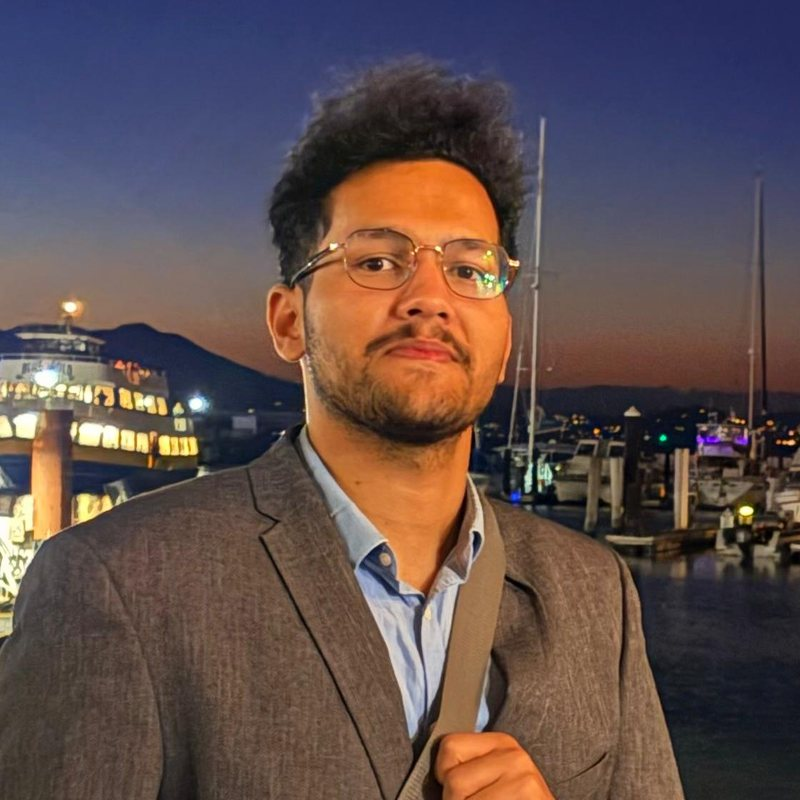
\includegraphics[width=2.5cm]{photo.jpg}};\end{tikzpicture}
\end{minipage}
\vspace{8pt}

{\color{accent!35}\rule{\textwidth}{.6pt}}\par\vspace{5pt}
I am developing algorithms for reconstructing attenuation maps from detector-scattered coincidences in PET imaging, enabling CT-less PET across the J-PET scanner family. Interests: image reconstruction, Monte Carlo simulation, deep learning for medical imaging, and PET detector instrumentation.

\section{Education}
\entry{PhD in Biophysics, Jagiellonian University, Kraków}{Oct 2024 -- 2028 (expected)}{J-PET Group \textbullet\ Supervisors: Prof.\ Pawe{\l} Moskal \& Dr.\ Sushil K.\ Sharma}{Thesis topic: CT-less PET imaging with the J-PET scanner using detector-scattered photons.}
\entry{MSc in Physics, Indian Institute of Technology Bombay}{2022 -- 2024}{CPI 8.12/10 \textbullet\ Supervisor: Prof.\ Pragya Das}{Projects: scattered data for tumour localisation in PET (2D TOF model); 3D annihilation-point estimation for PET reconstruction.}
\entry{BSc (Hons.) in Physics, Kirori Mal College, University of Delhi}{2019 -- 2022}{CGPA 9.42/10}{}

\section{Research Experience}
\entry{Doctoral Researcher, J-PET Group, Jagiellonian University}{Oct 2024 -- present}{}{\vspace{-2pt}\begin{itemize}
\item Developing \textbf{Detector-Scattered Attenuation Correction (DSAC)}: attenuation maps from inter-detector scattered coincidences, without CT.
\item Joint reconstruction (DS-MLAA, MLTR), analytical blank-scan modelling and GATE/Monte Carlo studies across LYSO, BGO and plastic scanners.
\item Deep-learning denoising of attenuation maps; team member of the NCN \textbf{MAESTRO} project.
\end{itemize}}
\entry{Content Developer, Vizuara (EdTech start-up)}{Sep -- Dec 2022}{}{Animated K--12 physics and maths explainers with Manim.}

\section{Patent}
\begin{itemize}
\item \me, P.~Moskal, S.~K.~Sharma, E.~St{\k{e}}pie{\'n}, ``Generating Attenuation Map from Detector-Scattered Coincidence Events in Positron Emission Tomography,'' \emph{US Patent Application No.\ 19/859,844}, filed 2 Nov 2026; priority: Polish Patent Application No.\ P.457524 (29 Oct 2026). Applicant: Jagiellonian University. \textbf{Patent pending.}
\end{itemize}

\section{Publications}
{\small\color{mute}16 publications \textbullet\ full list: \href{https://koza.if.uj.edu.pl/staff/stiwari}{koza.if.uj.edu.pl/staff/stiwari}}\par
\sub{First-author}
\begin{enumerate}
\item \me, S.~K.~Sharma, P.~Moskal, ``Feasibility study of using detector-scattered photons for attenuation correction in CT-less PET imaging,'' \emph{Bio-Algorithms and Med-Systems 21, 13--20 (2025)}. \doi{https://doi.org/10.5604/01.3001.0055.4655}{10.5604/01.3001.0055.4655}
\end{enumerate}
\sub{Software}
\begin{enumerate}[resume]
\item \me, ``BiblioAudit: Automated Citation Integrity \& Verification Tool'' (v2.2.2) [Software], \emph{Zenodo} (2025). \texttt{pip install biblioaudit}. \doi{https://doi.org/10.5281/zenodo.18155557}{10.5281/zenodo.18155557}
\end{enumerate}
\sub{Co-authored (J-PET Collaboration)}
\begin{enumerate}[resume]
\item Pawe{\l} Moskal, \ldots, \me, et al., ``First-in-human quantum entanglement imaging,'' \emph{arXiv preprint (2026)}. \doi{https://arxiv.org/abs/2606.29421}{arXiv:2606.29421}
\item Magdalena Skurzok, \ldots, \me, et al., ``Experimental determination of the Dalitz plot for positronium decay using the J-PET detection system,'' \emph{Physics Letters B 882, 141018 (2026)}. \doi{https://koza.if.uj.edu.pl/staff/stiwari}{koza.if.uj.edu.pl}
\item Szymon Parzych, \ldots, \me, et al., ``Feasibility simulation study of positronium lifetime imaging with the Biograph Vision Quadra and J-PET tomographs,'' \emph{EJNMMI Physics 13, 102 (2026)}. \doi{https://doi.org/10.1186/s40658-026-00920-1}{10.1186/s40658-026-00920-1}
\item Sushil K. Sharma, \ldots, \me, et al., ``First direct determination of the pick-off contribution to the ortho-positronium decay rate,'' \emph{Physics Letters B 879, 140610 (2026)}. \doi{https://doi.org/10.1016/j.physletb.2026.140610}{10.1016/j.physletb.2026.140610}
\item Krzysztof Kacprzak, \ldots, \me, et al., ``Methodology for time and TOT calibration of a modular J-PET scanner with prompt gamma emitters $^{22}$Na and $^{44}$Sc,'' \emph{Bio-Algorithms and Med-Systems 22, 36 (2026)}. \doi{https://doi.org/10.5604/01.3001.0055.6703}{10.5604/01.3001.0055.6703}
\item Reimund Bayerlein, Manish Das, \ldots, \me, et al., ``Monte Carlo-based scatter correction for the plastic-based modular PET scanner J-PET,'' \emph{Physics in Medicine \& Biology 71, 075026 (2026)}. \doi{https://doi.org/10.1088/1361-6560/ae54fb}{10.1088/1361-6560/ae54fb}
\item Manish Das, \ldots, \me, et al., ``First positronium imaging using $^{44}$Sc with the J-PET scanner: a case study on the NEMA image quality phantom,'' \emph{IEEE Trans. Radiat. Plasma Med. Sci. 10(4), 593 (2026)}. \doi{https://doi.org/10.1109/TRPMS.2025.3621554}{10.1109/TRPMS.2025.3621554}
\item Manish Das, \ldots, \me, et al., ``First positronium lifetime imaging using $^{52}$Mn and $^{55}$Co with a plastic-based PET scanner,'' \emph{Scientific Reports 16, 16230 (2026)}. \doi{https://doi.org/10.1038/s41598-026-43965-z}{10.1038/s41598-026-43965-z}
\item Karol Kubat, \ldots, \me, et al., ``First ex-vivo positronium imaging of tissues with modular J-PET scanner using $^{44}$Sc radionuclide,'' \emph{Z. Med. Phys. 36, 357--365 (2026)}. \doi{https://doi.org/10.1016/j.zemedi.2026.03.004}{10.1016/j.zemedi.2026.03.004}
\item Neha Chug, \ldots, \me, et al., ``Studies of CPT symmetry in positronium decays with the 192 plastic strip J-PET detector,'' \emph{Physical Review D 113, 032003 (2026)}. \doi{https://doi.org/10.1103/wy7r-xgl9}{10.1103/wy7r-xgl9}
\item Alessio Porcelli, \ldots, \me, et al., ``$\mu$PPET: Investigating the muon puzzle with J-PET detectors,'' \emph{Universe 11, 180 (2025)}. \doi{https://doi.org/10.3390/universe11060180}{10.3390/universe11060180}
\end{enumerate}
\sub{Conference proceedings}
\begin{enumerate}[resume]
\item Manish Das, \ldots, \me, et al., ``First experimental demonstration of positronium lifetime imaging with $^{44}$Sc using the J-PET scanner,'' \emph{2025 IEEE NSS/MIC/RTSD, Yokohama}. \doi{https://doi.org/10.1109/NSS/MIC/RTSD57106.2025.11286751}{10.1109/NSS/MIC/RTSD57106.2025.11286751}
\item Keyvan Tayefi Ardebili, \ldots, \me, et al., ``Development of a cost-effective Total Body J-PET from plastic scintillators: definitive design,'' \emph{2025 IEEE NSS/MIC/RTSD, Yokohama}. \doi{https://doi.org/10.1109/NSS/MIC/RTSD57106.2025.11287221}{10.1109/NSS/MIC/RTSD57106.2025.11287221}
\item M. R{\"a}dler, \ldots, \me, et al., ``Simulation studies of a brain PET insert for the Total Body J-PET tomograph,'' \emph{2025 IEEE NSS/MIC/RTSD, Yokohama}. \doi{https://doi.org/10.1109/NSS/MIC/RTSD57106.2025.11286628}{10.1109/NSS/MIC/RTSD57106.2025.11286628}
\item Reimund Bayerlein, \ldots, \me, et al., ``Monte Carlo-based scatter correction for J-PET,'' \emph{2025 IEEE NSS/MIC/RTSD, Yokohama}. \doi{https://doi.org/10.1109/NSS/MIC/RTSD57106.2025.11287184}{10.1109/NSS/MIC/RTSD57106.2025.11287184}
\end{enumerate}

\section{Conference Contributions}
\row{\textbf{IEEE NSS/MIC/RTSD 2026}, Granada, Spain \textendash\ \emph{Poster} \textbullet\ \textbf{Trainee Grant}}{Nov 2026}
{\small\color{mute}\hspace{1.1em}A Comparative Simulation Study of DSAC for CT-less PET: LYSO vs Plastic vs BGO Scanners}\par\vspace{3pt}
\row{\textbf{Total-Body PET 2026}, UC Davis, USA \textendash\ \emph{Poster} \textbullet\ \textbf{Presentation Award} \textbullet\ Travel Grant}{Sep 2026}
{\small\color{mute}\hspace{1.1em}CT-less Attenuation Correction Using Detector-Scattered Photons in Plastic-Scintillator Total-Body PET: A Monte Carlo Study}\par\vspace{3pt}
\row{\textbf{6th Jagiellonian Symposium}, Kraków \textendash\ \emph{Talk} \textbullet\ core organiser}{Jul 2026}
{\small\color{mute}\hspace{1.1em}Analytical Modelling of Blank Scan in Detector-Scattered Attenuation Correction (DSAC)}\par\vspace{3pt}
\row{\textbf{MCSB 2026}, Kraków \textendash\ \emph{Talk}}{May 2026}
{\small\color{mute}\hspace{1.1em}Deep-learning enhancement of detector-scatter attenuation maps for CT-less plastic-scintillator PET}\par\vspace{3pt}
\row{\textbf{FTMI-TBPET-PSMR 2026}, Valencia, Spain \textendash\ \emph{Talk}}{May 2026}
{\small\color{mute}\hspace{1.1em}DSAC: A Novel CT-less Attenuation Correction Approach for Cost-Effective Plastic-Scintillator Total-Body PET}\par\vspace{3pt}
\row{\textbf{EMIM 2026}, Ljubljana, Slovenia \textendash\ \emph{Poster}}{Mar 2026}
{\small\color{mute}\hspace{1.1em}CT-less Attenuation Correction via ML Reconstruction (DS-MLAA)}\par\vspace{3pt}
\row{\textbf{2nd Total-Body J-PET General Meeting}, Kraków \textendash\ \emph{Talk} \textbullet\ core organiser}{Jan 2026}
\row{\textbf{2nd Symposium on New Trends in Nuclear \& Medical Physics}, Kraków \textendash\ \emph{Poster} \textbullet\ organiser}{Sep 2025}
\row{\textbf{1st Total-Body J-PET General Meeting}, Kraków \textendash\ \emph{Talk}}{Oct 2024}
\sub{Schools}
\row{AI in Medical Imaging Summer School, Radboud University, Nijmegen}{Jun -- Jul 2025}

\section{Awards \& Grants}
\row{\textbf{Trainee Grant}, IEEE NSS/MIC/RTSD 2026 (registration fee covered)}{Nov 2026}
\row{\textbf{Presentation Award}, Total-Body PET 2026, UC Davis}{Sep 2026}
\row{\textbf{Travel Grant}, Total-Body PET 2026, UC Davis}{Sep 2026}
\row{\textbf{TD-UJ Research Grant} (\(\times\)3), Jagiellonian University}{Jun 2024 \textbullet\ Apr 2026 \textbullet\ Sep 2026}
\row{\textbf{STER Mobility Grant}, NAWA (international research internship)}{2026}
\row{\textbf{Visibility \& Mobility Grant}, ID UJ}{Apr 2026}
\row{\textbf{PROM Mobility Grant}, NAWA}{Feb 2025}
\row{\textbf{All India Rank 15}, IIT JAM Physics}{Mar 2022}
\row{\textbf{National Topper (top 1\%)}, National Graduate Physics Examination, IAPT}{May 2022}

\section{Teaching \& Service}
\row{\textbf{Teaching Assistant}, Jagiellonian University \textendash\ Monte Carlo methods lectures; Python for beginners}{}
\row{\textbf{Peer Reviewer}, \emph{EJNMMI Physics}; \emph{Bio-Algorithms and Med-Systems}}{2026 -- present}
\row{\textbf{Doctoral Council Representative}, Biophysics PhD students, Jagiellonian University}{2025 -- 2026}
\row{\textbf{TD-UJ Interdisciplinary Team}: Research Salons, seminars; Housing Committee}{2025 -- 2026}
\row{\textbf{Department Coordinator}, ISCP, IIT Bombay: PG orientation for 1500+ students; mentored 7 juniors}{2023 -- 2024}

\section{Skills}
\begin{tabularx}{\textwidth}{@{}>{\bfseries\raggedright\arraybackslash}p{4.1cm}X@{}}
Imaging \& simulation & GATE/Geant4, Monte Carlo, iterative reconstruction (MLAA, MLTR), ROOT\\
Programming & Python, C++, SQL, Fortran, Mathematica, MATLAB\\
Machine learning & TensorFlow, scikit-learn, NumPy, Pandas\\
Certifications & Fast-timing Scintillation Detectors for Medical Applications; Machine Learning Specialization (Andrew Ng); Neural Networks \& Deep Learning (DeepLearning.AI)\\
\end{tabularx}

\section{References}
\begin{tabularx}{\textwidth}{@{}X X@{}}
\textbf{Prof.\ dr hab.\ Pawe{\l} Moskal} (PhD supervisor) & \textbf{Dr.\ Sushil K.\ Sharma} (PhD co-supervisor)\\
Head, Cluster of Nuclear Physics Departments; J-PET group leader, Jagiellonian University & Assistant Professor, Institute of Physics, Jagiellonian University\\
\href{mailto:p.moskal@uj.edu.pl}{p.moskal@uj.edu.pl} & \href{mailto:sushil.sharma@uj.edu.pl}{sushil.sharma@uj.edu.pl}\\
\end{tabularx}
\end{document}
